\section{Penman model (model ID: 17)}
The Penman model (fig.~\ref{fig:17_schematic}) is based on the drying curve concept described in \citet{PENMAN1950} \citep{Wagener2002}. It has 3 stores and 4 parameters ($S_{max}$, $\phi$, $\gamma$, $k_1$). The model aims to represent:

\begin{itemizecompact}
\item Moisture accumulation and evaporation from the root zone;
\item Bypass of excess moisture to the stream;
\item Deficit-based groundwater accounting;
\item Linear flow routing.
\end{itemizecompact}

\subsection{MARRMoT model name}
m\_17\_penman\_4p\_3s \\

% Equations
\subsection{Model equations}

% Model layout figure
{ 																	% This ensures it doesn't warp text further down
\begin{wrapfigure}{l}{4.5cm}
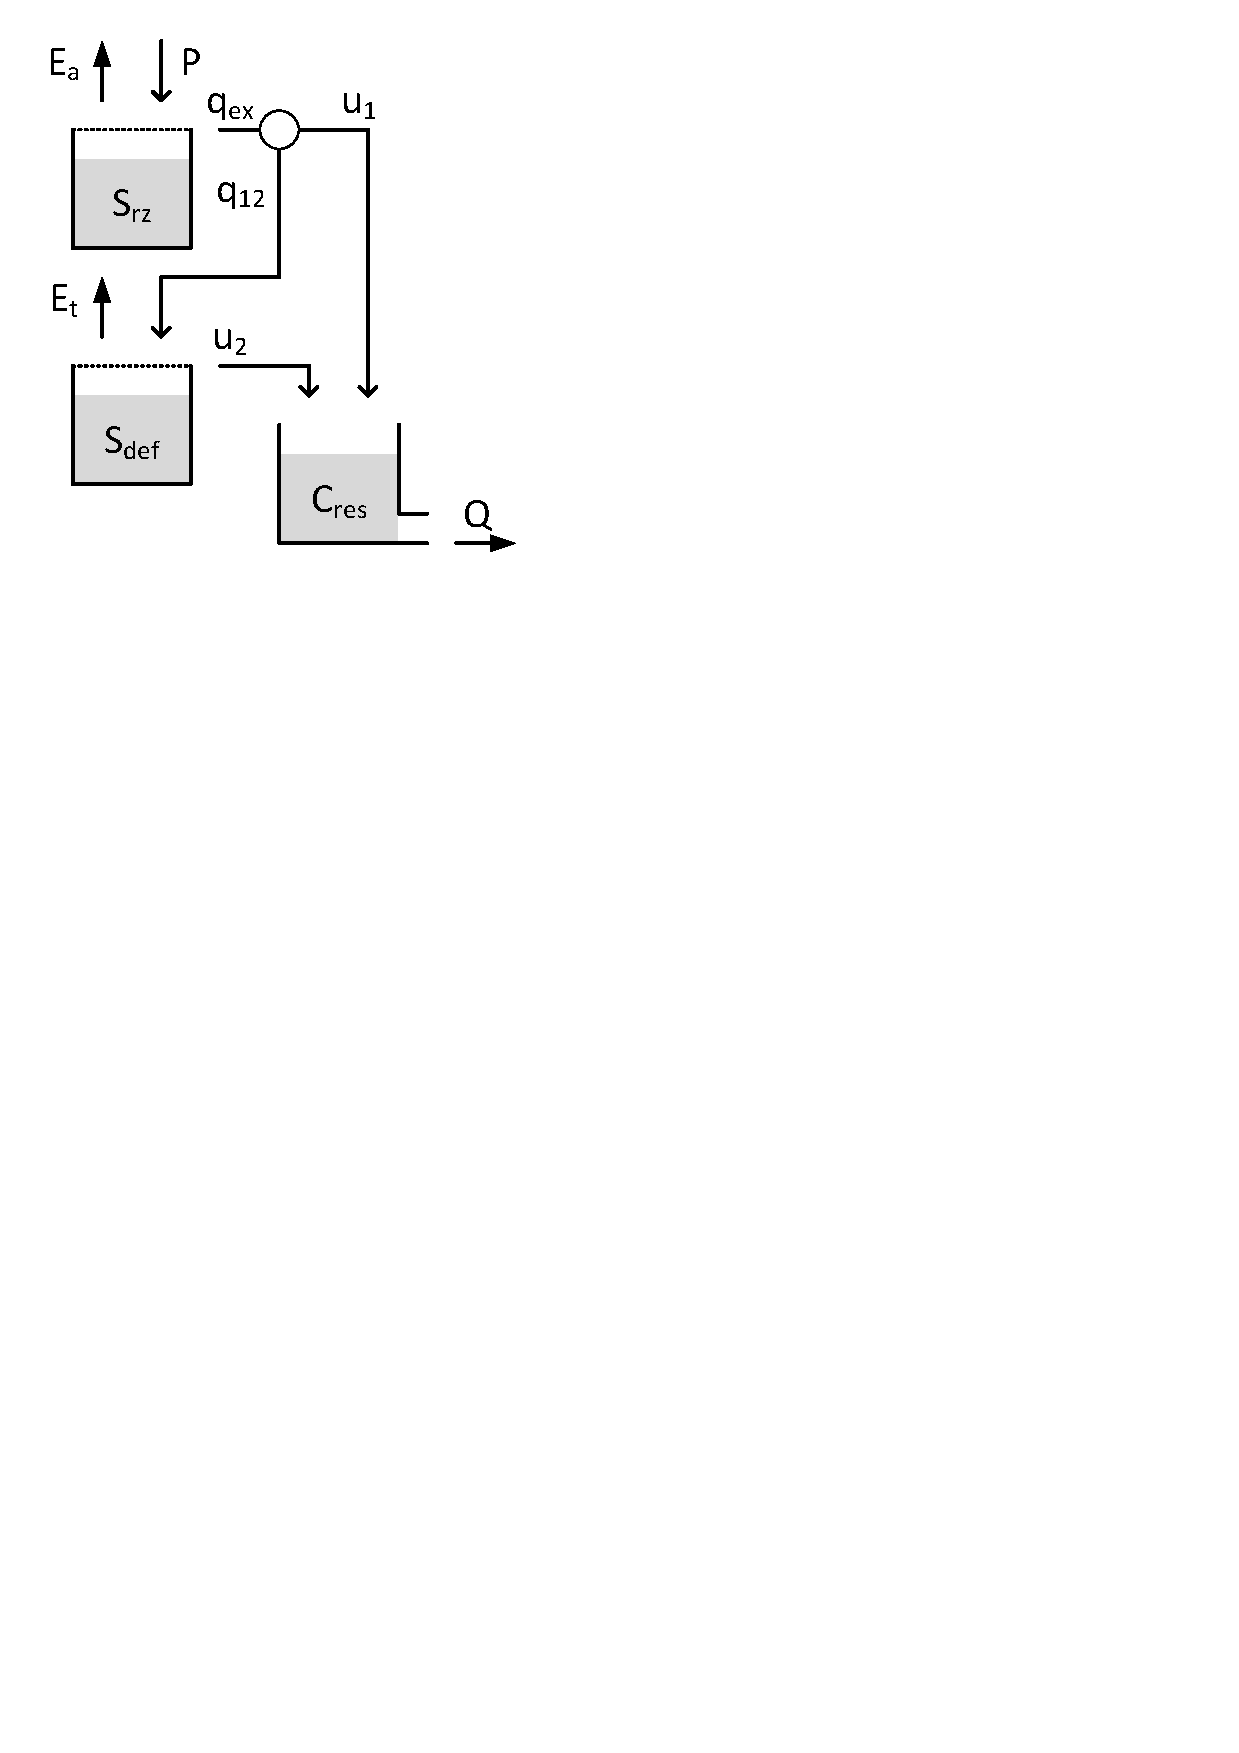
\includegraphics[trim=1cm 20cm 7cm 1cm,width=7cm,keepaspectratio]{./AppA_files/17_schematic.pdf}
\caption{Structure of the Penman model} \label{fig:17_schematic}
\end{wrapfigure}

\begin{align}
	\frac{dS_{rz}}{dt} &= P-E_a-q_{ex} \\
	E_a &= \begin{cases}
		E_p, &\text{if } S_{rz} > 0 \\
		0, & \text{otherwise} \\
	\end{cases} \\
	q_{ex} &= 
	\begin{cases}
		P, & \text{if } S_{rz} = S_{max} \\
		0, & \text{otherwise}
	\end{cases}
\end{align}

Where $S_{rz}$ [mm] is the current storage in the root zone, refilled by precipitation $P$ $[mm/d]$ and drained by evaporation $E_a$  $[mm/d]$ and moisture excess $q_{ex}$  $[mm/d]$. $E_a$ occurs at the potential rate $E_p$  $[mm/d]$ whenever possible. $q_{ex}$ occurs only when the store is at maximum capacity $S_{max}$ [mm].

} % end of wrapfigure fix

\begin{align}
	\frac{dS_{def}}{dt} &= E_t+u_2-q_{12}\\
	E_t &= \begin{cases}
		\gamma*E_p, &\text{if } S_{rz} = 0 \\
		0, &\text{otherwise} \\
	\end{cases} \\
	u_2 &= \begin{cases}
		q_{12}, &\text{if } S_{def} = 0\\
		0, &\text{otherwise}\\
	\end{cases}	\\
	q_{12} &= (1-\phi)*q_{ex}
\end{align}

Where $S_{def}$ [mm] is the current moisture \emph{deficit}, which is increased by evaporation $E_t$ $[mm/d]$ and reduced by inflow $q_{12}$ $[mm/d]$. 
$E_t$ occurs only when the upper store $S_{rz}$ is empty and at a fraction $\gamma$ [-] of $E_p$. 
Inflow $q_{12}$ is the fraction $(1-\phi)$ [-] of $q_{ex}$ that does not bypass the lower soil layer. 
Saturation excess $u_2$ $[mm/d]$ occurs only when there is zero deficit.

\begin{align}
	\frac{dC_{res}}{dt} &= u_1+u_2-Q\\
	u_1 &= \phi*q_{ex}\\
	Q &= k_1*C_{res}
\end{align}
  
Where $C_{res}$ [mm] is the current storage in the routing reservoir, increased by $u_1$ and $u_2$, and drained by runoff $Q$  $[mm/d]$. $u_1$ is the fraction $\phi$ of $q_{ex}$. $Q$ has a linear relationship with storage through time scale parameter $k_1$ $[d^{-1}]$.

\subsection{Parameter overview}

% Table generated by Excel2LaTeX from sheet 'Sheet1'
\begin{table}[htbp]
  \centering
    \begin{tabular}{lll}
    \toprule
    Parameter & Unit  & Description \\
    \midrule
    $S_{max}$ & $mm$  & Maximum soil moisture storage \\
    $\phi$ & $-$   & Fraction of saturation excess that is direct runoff \\
    $\gamma$ & $-$   & Evaporation reduction factor \\
    $k_1$ & $d^{-1}$ & Runoff coefficient \\
    \bottomrule
    \end{tabular}%
  \label{tab:addlabel}%
\end{table}%


